
% this file is called up by thesis.tex
% content in this file will be fed into the main document

%: ----------------------- introduction file header -----------------------
\chapter{Future Work and Conclusions}

% the code below specifies where the figures are stored
\ifpdf
    \graphicspath{{11_future_work_and_conclusions/figures/PNG/}{11_future_work_and_conclusions/figures/PDF/}{11_future_work_and_conclusions/figures/}}
\else
    \graphicspath{{11_future_work_and_conclusions/figures/EPS/}{11_future_work_and_conclusions/figures/}}
\fi

% ----------------------------------------------------------------------
%: ------------------------------- content ----------------------------- 
% ----------------------------------------------------------------------

\begin{figure}
  \centering
  \includegraphics[width=\linewidth]{seen.png}
  \caption{Mahaya's commercial automatic event archiving tool Seen
    (\url{http://mahaya.co/})}
  \label{fig:seen}
\end{figure}

\begin{figure}
  \centering
  \includegraphics[width=\linewidth]{eventifier.png}
  \caption{The automatic commercial event archiving tool Eventifier
    (\url{http://eventifier.co/})}
  \label{fig:eventifier}
\end{figure}

\begin{figure}
  \centering
  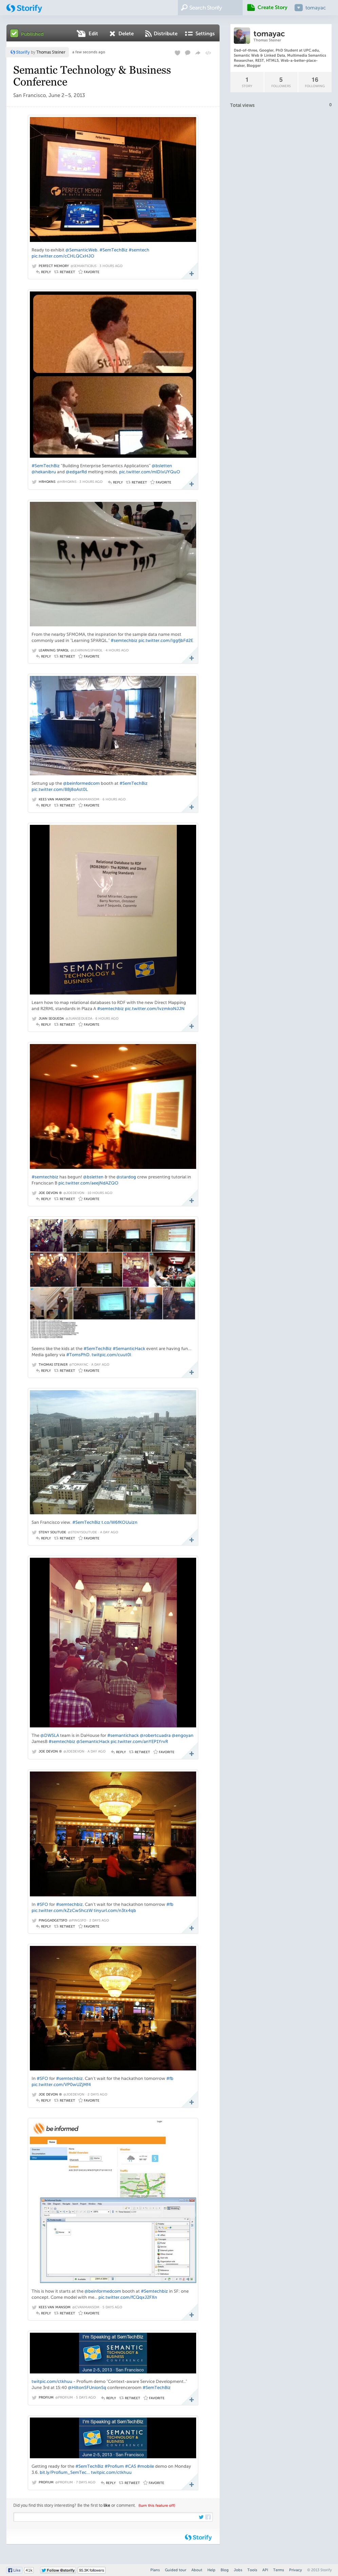
\includegraphics[width=\linewidth]{storify.png}
  \caption{The manual assisted commercial event archiving tool Storify
    (\url{http://storify.com/})}
  \label{fig:storify}
\end{figure}

\begin{figure}
  \centering
  \includegraphics[width=\linewidth]{mediafinder.png}
  \caption{The academic event summarization tool Media Finder}
  \label{fig:mediafinder}
\end{figure}

\begin{figure}
  \centering
  \includegraphics[width=\linewidth]{socialmediaillustrator.png}
  \caption{Our own academic event summarization tool Social Media Illustrator}
  \label{fig:socialmediaillustrator}
\end{figure}

The research fields of event summarization and event archiving
based on social network multimedia data have resulted in 
interesting business creations in recent months.
Albeit similarities to our work exist,
there are still many differences in the details.
The company Mahaya has launched a~beta event archiving tool called Seen,
which, based on manually entered event metadata like event name,
location, and dates, uses the necessarily provided Twitter hashtag
to create a~complete archive of all event-related tweets,
media items, slide and decks.
Based on term occurrence frequency and co-occurrence analysis,
the event is split into subevents.


Credibility on Storyful.com \url{http://www.ted.com/talks/markham_nolan_how_to_separate_fact_and_fiction_online.html}

\section{Contributions}

\section{Research Directions}





